
\subsection{Dostava paketa}
\begin{figure}[h]
	\begin{center}
		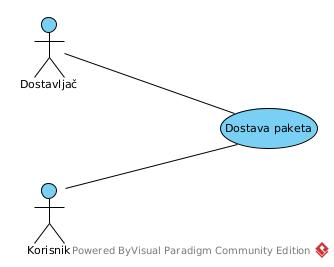
\includegraphics[scale=0.8]{uc_package_delivery}
	\end{center}
	\caption{Dijagram slučajeva upotrebe dostave paketa}
%	\label{fig:UCPackageDelivery}
\end{figure}

	\begin{itemize}
		\item{Kratak opis:} 
		
		- Dostavljač dobija informacije o paketu od sistema i dostavlja paket korisniku.
		\item{Učesnici:} 
		
		- Dostavljač, korisnik
		\item{Preduslovi:}
		
		- Dostavljač je prijavljen na sistem i ima nedostavljenih paketa. Korisnik je na registrovanoj adresi u vreme dostave.
		\item{Postuslovi:}
		
		- Korisnik dobija svoj paket sa namirnicama
		\item{Osnovni tok:}
		\begin{enumerate}
			\item{Dostavljač dobija obaveštenje od sistema da ima nedostavljenih paketa.}
			\item{Dostavljač dolazi do magacina gde su smešteni paketi.}
			\item{Dostavljač očitava identifikacioni broj paketa pomoću sistema i dobija informacije o porudžbini.}
			\item{Dostavljač dolazi do destinacije korisnika u predviđenom periodu.}
			\item{Korisnik preuzima svoj paket.}
			\item{Dostavljač beleži da je uspešno izvršio dostavu.}

			\textit{Koraci 2-6 se ponavljaju sve dok ima nedostavljenih paketa.}
		\end{enumerate}
		
		\item{Alternativni tokovi:}
			\begin{enumerate}
				\item[A1.] \textbf{Dostavljač kasni sa dostavom.} Ukoliko u koraku 4 				dostavljač proceni da će kasniti, obaveštava korisnika pomoću sistema.
%				\item[A2.] \textbf{Korisnik se trenutno ne nalazi na naznačenoj adresi.} Ukoliko u koraku 5 korisnik nije na naznačenoj adresi, dostavljač beleži da je dostava neuspela i vraća paket u magacin. Sistem obaveštava korisnika da dostavljač nije uspeo da dostavi paket i traži od korisnika da potvrdi svoju adresu. Ako je korisnik promenio adresu, sistem ga navodi na opciju ažuriranja naloga.  
			\end{enumerate}
	\end{itemize}
	
\begin{figure}[h]
	\begin{center}
		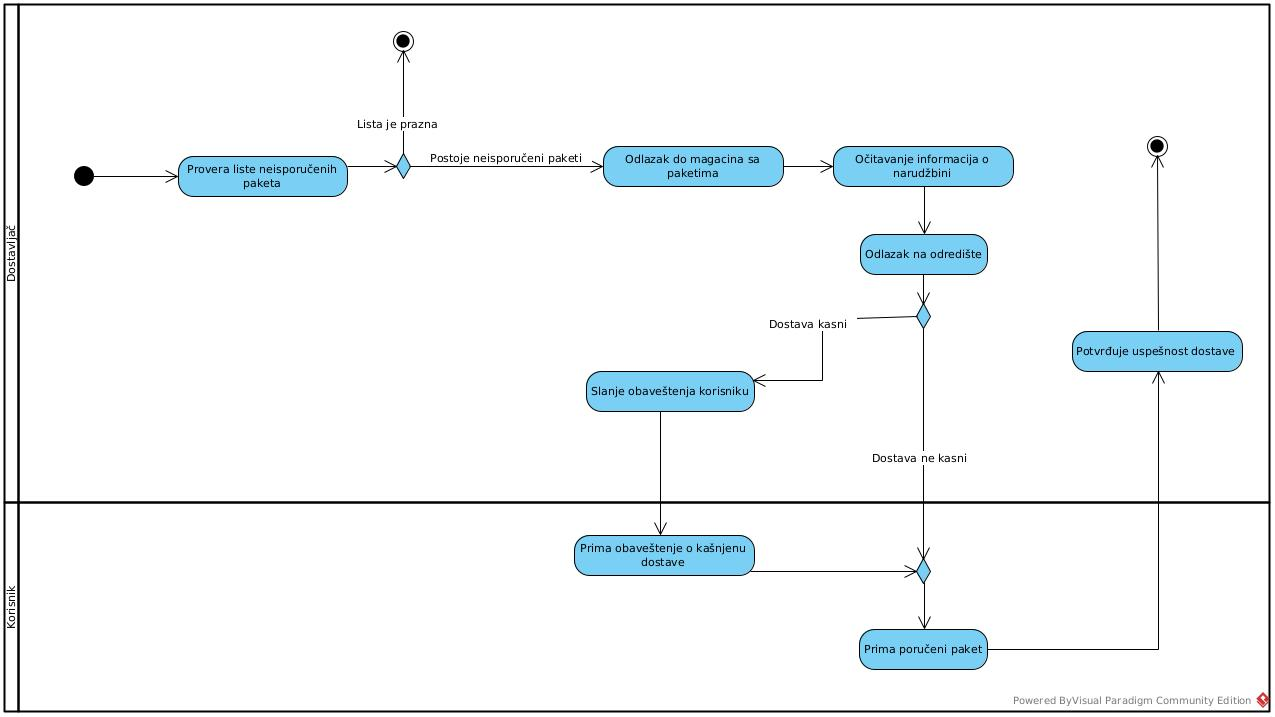
\includegraphics[width=1\textwidth]{activity_package_delivery}
	\end{center}
	\caption{Dijagram aktivnosti dostave paketa}
%	\label{fig:UCPackageDelivery}
\end{figure}	
